\documentclass[journal,article,submit,moreauthors,pdftex,10pt,a4paper]{Definitions/mdpi} 
\usepackage{algorithm}
\usepackage{algorithmicx}
\usepackage{amsmath}
\usepackage{algpseudocode}
\renewcommand{\algorithmicrequire}{\textbf{Input:}}  % Use Input in the format of Algorithm
\renewcommand{\algorithmicensure}{\textbf{Output:}} % Use Output in the format of Algorithm
\usepackage{amsthm}
\usepackage{amsmath}
\usepackage{enumitem}
\usepackage{color} %red, green, blue, yellow, cyan, magenta, black, white
\definecolor{mygreen}{RGB}{28,172,0} % color values Red, Green, Blue
\definecolor{mylilas}{RGB}{170,55,241}
\newlist{steps}{enumerate}{1}
\setlist[steps, 1]{label = Step \arabic*).}
\theoremstyle{plain}
\newtheorem{thm}{Theorem}[section]
\newtheorem{lem}[thm]{Lemma}
\newtheorem{prop}[thm]{Proposition}
\newtheorem*{cor}{Corollary}

\theoremstyle{definition}
\newtheorem{defn}{Definition}[section]
\newtheorem{conj}{Conjecture}[section]
\newtheorem{exmp}{Example}[section]

\theoremstyle{remark}
\newtheorem*{rem}{Remark}
\newtheorem*{note}{Note}
% If you would like to post an early version of this manuscript as a preprint, you may use preprint as the journal and change 'submit' to 'accept'. The document class line would be, e.g., \documentclass[preprints,article,accept,moreauthors,pdftex,10pt,a4paper]{mdpi}. This is especially recommended for submission to arXiv, where line numbers should be removed before posting. For preprints.org, the editorial staff will make this change immediately prior to posting.

%
%--------------------
% Class Options:
%--------------------
% journal
%----------
% Choose between the following MDPI journals:
% acoustics, actuators, addictions, admsci, aerospace, agriculture, agronomy, algorithms, animals, antibiotics, antibodies, antioxidants, applsci, arts, asi, atmosphere, atoms, axioms, batteries, bdcc, behavsci, beverages, bioengineering, biology, biomedicines, biomimetics, biomolecules, biosensors, brainsci, buildings, carbon, cancers, catalysts, cells, ceramics, challenges, chemengineering, chemosensors, children, cleantechnol, climate, clockssleep, cmd, coatings, colloids, computation, computers, condensedmatter, cosmetics, cryptography, crystals, cybersecurity, data, dentistry, designs, diagnostics, dairy, diseases, diversity, drones, econometrics, economies, education, electrochem, electrochemistry, electronics, energies, entropy, environments, epigenomes, est, fermentation, fibers, fire, fishes, fluids, foods, forecasting, forests, fractalfract, futureinternet, galaxies, games, gastrointestdisord, gels, genealogy, genes, geohazards, geosciences, geriatrics, hazardousmatters, healthcare, heritage, highthroughput, horticulturae, humanities, hydrology, informatics, information, infrastructures, inorganics, insects, instruments, ijerph, ijfs, ijms, ijgi, ijtpp, inventions, j, jcdd, jcm, jcs, jdb, jfb, jfmk, jimaging, jof, jintelligence, jlpea, jmmp, jmse, jpm, jrfm, jsan, land, languages, laws, life, literature, logistics, lubricants, machines, magnetochemistry, make, marinedrugs, materials, mathematics, mca, medsci, medicina, medicines, membranes, metabolites, metals, microarrays, micromachines, microorganisms, minerals, modelling, molbank, molecules, mps, mti, nanomaterials, ncrna, neonatalscreening, neuroglia, nitrogen, nutrients, ohbm, particles, pathogens, pharmaceuticals, pharmaceutics, pharmacy, philosophies, photonics, plants, plasma, polymers, polysaccharides, proceedings, processes, proteomes, publications, quaternary, qubs, reactions, recycling, religions, remotesensing, reports, resources, risks, robotics, safety, sci, scipharm, sensors, separations, sexes, sinusitis, smartcities, socsci, societies, soilsystems, sports, standards, stats, surfaces, surgeries, sustainability, symmetry, systems, technologies, toxics, toxins, tropicalmed, universe, urbansci, vaccines, vehicles, vetsci, vibration, viruses, vision, water, wem, wevj
%---------
% article
%---------
% The default type of manuscript is article, but can be replaced by: 
% abstract, addendum, article, benchmark, book, bookreview, briefreport, casereport, changes, comment, commentary, communication, conceptpaper, correction, conferenceproceedings, conferencereport, expressionofconcern, extendedabstract, meetingreport, creative, datadescriptor, discussion, editorial, essay, erratum, hypothesis, interestingimages, letter, meetingreport, newbookreceived, opinion, obituary, projectreport, reply, reprint, retraction, review, perspective, protocol, shortnote, supfile, technicalnote, viewpoint
% supfile = supplementary materials
% protocol: If you are preparing a "Protocol" paper, please refer to http://www.mdpi.com/journal/mps/instructions for details on its expected structure and content.
%----------
% submit
%----------
% The class option "submit" will be changed to "accept" by the Editorial Office when the paper is accepted. This will only make changes to the frontpage (e.g., the logo of the journal will get visible), the headings, and the copyright information. Also, line numbering will be removed. Journal info and pagination for accepted papers will also be assigned by the Editorial Office.
%------------------
% moreauthors
%------------------
% If there is only one author the class option oneauthor should be used. Otherwise use the class option moreauthors.
%---------
% pdftex
%---------
% The option pdftex is for use with pdfLaTeX. If eps figures are used, remove the option pdftex and use LaTeX and dvi2pdf.

%=================================================================
\firstpage{1} 
\makeatletter 
\setcounter{page}{\@firstpage} 
\makeatother
\pubvolume{xx}
\issuenum{1}
\articlenumber{5}
\pubyear{2018}
\copyrightyear{2018}
%\externaleditor{Academic Editor: name}
\history{Received: date; Accepted: date; Published: date}
%\updates{yes} % If there is an update available, un-comment this line

%% MDPI internal command: uncomment if new journal that already uses continuous page numbers 
%\continuouspages{yes}

%------------------------------------------------------------------
% The following line should be uncommented if the LaTeX file is uploaded to arXiv.org
%\pdfoutput=1

%=================================================================
% Add packages and commands here. The following packages are loaded in our class file: fontenc, calc, indentfirst, fancyhdr, graphicx, lastpage, ifthen, lineno, float, amsmath, setspace, enumitem, mathpazo, booktabs, titlesec, etoolbox, amsthm, hyphenat, natbib, hyperref, footmisc, geometry, caption, url, mdframed, tabto, soul, multirow, microtype, tikz

%=================================================================
%% Please use the following mathematics environments: Theorem, Lemma, Corollary, Proposition, Characterization, Property, Problem, Example, ExamplesandDefinitions, Hypothesis, Remark, Definition
%% For proofs, please use the proof environment (the amsthm package is loaded by the MDPI class).

%=================================================================
% Full title of the paper (Capitalized)
\Title{Efficient Tensor Sensing For RF Tomographic Imaging on GPUs}

% Author Orchid ID: enter ID or remove command
\newcommand{\orcidauthorA}{0000-0000-000-000X} % Add \orcidA{} behind the author's name
%\newcommand{\orcidauthorB}{0000-0000-000-000X} % Add \orcidB{} behind the author's name

% Authors, for the paper (add full first names)
\Author{Tao Zhang $^{1,\dagger,\ddagger}$\orcidA{}, Da Xu $^{1,\ddagger}$ and Firstname Lastname $^{2,}$*}

% Authors, for metadata in PDF
\AuthorNames{Firstname Lastname, Firstname Lastname and Firstname Lastname}

% Affiliations / Addresses (Add [1] after \address if there is only one affiliation.)
\address{%
$^{1}$ \quad Affiliation 1; e-mail@e-mail.com\\
$^{2}$ \quad Affiliation 2; e-mail@e-mail.com}

% Contact information of the corresponding author
\corres{Correspondence: e-mail@e-mail.com; Tel.: +x-xxx-xxx-xxxx}

% Current address and/or shared authorship
\firstnote{Current address: Affiliation 3} 
\secondnote{These authors contributed equally to this work.}
% The commands \thirdnote{} till \eighthnote{} are available for further notes

%\simplesumm{} % Simple summary

%\conference{} % An extended version of a conference paper

% Abstract (Do not insert blank lines, i.e. \\) 
\abstract{Radio-frequency(RF)tomographic imaging is a promising technique for inferring multi-dimensional physical space by processing RF signals traversed across a region of interest.
The transform-based tensor model is more considered to be more appropriate than conventional model based on vector. The Alt-Min approach proposed by Deng. demonstrate significanct
improvement in recovery error and convergence sppeed compared to prior tensor-based compressed sensing. However, the running time of Tubal-Alt-Min increases exponentially with the dimension of 
tensors, thus not very practical for medium- or large-scale tensors. In this paper, we address this problem by exploiting massively parallel GPUs. We design, implement and optimize the 
Alt-Min algorithm on a GPU and evaluate the performance in terms of running time, recovery error, and convergence speed. }
%Experiment results show that the GPU algorithm is as accurate as the CPU counterpart with 63.69x speedup on average for all tensor sizes and up to 108.88x for large  tensors. We further encapsulate the GPU algorithm into an open-source library, called \textit{cuTensor}, and demonstrate its application in video data recovery. The cuTensor library can be easily applied on many other applications of tensor completion.}

% Keywords
\keyword{keyword 1; keyword 2; keyword 3 (list three to ten pertinent keywords specific to the article, yet reasonably common within the subject discipline.)}

% The fields PACS, MSC, and JEL may be left empty or commented out if not applicable
%\PACS{J0101}
%\MSC{}
%\JEL{}

%%%%%%%%%%%%%%%%%%%%%%%%%%%%%%%%%%%%%%%%%%
% Only for the journal Diversity
%\LSID{\url{http://}}

%%%%%%%%%%%%%%%%%%%%%%%%%%%%%%%%%%%%%%%%%%
% Only for the journal Applied Sciences:
%\featuredapplication{Authors are encouraged to provide a concise description of the specific application or a potential application of the work. This section is not mandatory.}
%%%%%%%%%%%%%%%%%%%%%%%%%%%%%%%%%%%%%%%%%%

%%%%%%%%%%%%%%%%%%%%%%%%%%%%%%%%%%%%%%%%%%
% Only for the journal Data:
%\dataset{DOI number or link to the deposited data set in cases where the data set is published or set to be published separately. If the data set is submitted and will be published as a supplement to this paper in the journal Data, this field will be filled by the editors of the journal. In this case, please make sure to submit the data set as a supplement when entering your manuscript into our manuscript editorial system.}

%\datasetlicense{license under which the data set is made available (CC0, CC-BY, CC-BY-SA, CC-BY-NC, etc.)}

%%%%%%%%%%%%%%%%%%%%%%%%%%%%%%%%%%%%%%%%%%
% Only for the journal Toxins
%\keycontribution{The breakthroughs or highlights of the manuscript. Authors can write one or two sentences to describe the most important part of the paper.}

%\setcounter{secnumdepth}{4}
%%%%%%%%%%%%%%%%%%%%%%%%%%%%%%%%%%%%%%%%%%
\begin{document}
%%%%%%%%%%%%%%%%%%%%%%%%%%%%%%%%%%%%%%%%%%
%% Only for the journal Gels: Please place the Experimental Section after the Conclusions

%%%%%%%%%%%%%%%%%%%%%%%%%%%%%%%%%%%%%%%%%%
\setcounter{section}{-1} %% Remove this when starting to work on the template.
\section{How to Use this Template}
The template details the sections that can be used in a manuscript. Note that the order and names of article sections may differ from the requirements of the journal (e.g., the positioning of the Materials and Methods section). Please check the instructions for authors page of the journal to verify the correct order and names. For any questions, please contact the editorial office of the journal or support@mdpi.com. For LaTeX related questions please contact Janine Daum at latex-support@mdpi.com.
%The order of the section titles is: Introduction, Materials and Methods, Results, Discussion, Conclusions for these journals: aerospace,algorithms,antibodies,antioxidants,atmosphere,axioms,biomedicines,carbon,crystals,designs,diagnostics,environments,fermentation,fluids,forests,fractalfract,informatics,information,inventions,jfmk,jrfm,lubricants,neonatalscreening,neuroglia,particles,pharmaceutics,polymers,processes,technologies,viruses,vision

\section{Introduction}

\section{Related Work}
There are quite a lot of work on the reconstruction of RF tomography, which can be classified into vector-based and tensor-based methods.
The vector-based RF tomography compression sensing methods are proposed in \cite{kanso2009compressed, mostofi2011compressive}. However, these methods can only infer two-dimensional space because they ignore the spatial structure of the data. 
The tensor-based approach is proposed in \cite{matsuda2017multi}, which uses tensor nuclear norm(TNN) \cite{li2013generalized} to extend RF tomographic problems to three-dimensional case. The method requires tensor singular value decomposition(t-SVD) , which is high computational complexity. Furthermore, the recovery error of this method is relatively high and the size of the data that can be processed is too small for the actual scene.Reference \cite{}uses a transform-based tensor model\cite{liu2017fourth} to efficiently explore three-dimensional spatial structures for higher accuracy and efficiency. 

Many existing researches \cite{jing2016energy} \cite{zhang2015buddy} \cite{zhang2015efficient} \cite{zhang2014cuirre} \cite{zhang2016efficient} have demonstrated the benefit of utilizing GPUs to accelerate general purpose computing. Because of the massive parallelism and high memory bandwidth, GPUs are often used in accelerating machine learning applications \cite{chetlur2014cudnn} \cite{tsung2016high} \cite{banasiak2016statistical}.  Recently it has been applied to accelerate tensor contractions \cite{shi2016tensor} and the proposed new BLAS-like primitive called STRIDEDBATCHEDGEMM is capable of performing a wide range of tensor contractions on CPU and GPU efficiently. Sparse tensor-times-dense matrix multiply is a critical bottleneck in data analysis and mining applications and \cite{li2016optimizing} proposed an efficient primitive on CPU and GPU platforms. Solving large numbers of small linear algebra problems simultaneously is becoming increasingly important in many application areas and \cite{dongarra2017optimized} made a systematic work to optimize batched linear algebra for GPUs.

%%%%%%%%%%%%%%%%%%%%%%%%%%%%%%%%%%%%%%%%%%
\section{Notations and Tensor Sensing Problem}
    We first formulate the RF tomographic imaging task as a tensor sensing problem, then review the Alt-Min algorithm. 

\subsection{Notations and the Transform-based Tensor Model}
We use lowercase boldface letter $\mathbf{x} \in \mathbb{R}^{N_1}$ to denote a vector, uppercase boldface letter $\mathbf{X} \in \mathbb{R}^{N_1 \times N_2}$ to denote a matrix, 
and calligraphic letter $\mathcal{X} \in \mathbb{R}^{N_1 \times N_2 \times N_3}$ to denote a tensor. $[k]$ denotes the set $\{1,2,\dots, k\}$. Let $\mathcal{A} \in \mathbb{R}^{N_1 \times N_2 \times N_3}$ 
denote a thirdorder tensor. $\mathcal{A}(:,j,k)$, $\mathcal{A}(i,:,k)$, $\mathcal{A}(i,j:)$ denote mode-1, mode-2, mode-3 tubes of $\mathcal{A}$, and $\mathcal{A}(:,:,k)$, $\mathcal{A}(:,j,:)$ $\mathcal{A}(i,:,:)$ 
denote the frontal, lateral, and horizontal slices. The Frobenius norm of $\mathcal{A}$ is defined as $\|\mathcal{A}\|_F = \sqrt{\sum ^{N_1}_{i = 1} \sum ^{N_2}_{j = 1} \sum ^{N_3}_{k = 1} \mathcal{A}^2_{ijk}}$.
The operator vec(.) transforms tensors and matrices into vectors. Let $\mathbf{X}^{T}$ and $\mathcal{A}^{\dagger}$ denote the transposes of a matrix and a tensor, respectively.
\begin{defn}\cite{liu2017fourth}
    Given an invertible discrete transform $\mathcal{L}:\mathbb{R}^{1\times 1 \times N_3} \to \mathbb{R}^{1\times 1\times N_3}$, the elementwise multiplication $\circ$, and $\mathbf{a}, \mathbf{b} \in \mathbb{R}^{1\times 1\times N_3}$ , the tubal-scalar multiplication is defined as:
        \begin{equation}
            \mathbf{a} \bullet \mathbf{b} = \mathcal{L}^{-1}(\mathcal{L}(\mathbf{a})\circ \mathcal{L}(\mathbf{b}))
        \end{equation}
\end{defn}

\begin{defn}\cite{liu2017fourth}
    The $\mathcal{L}$-product $\mathcal{A} = \mathcal{B} \bullet \mathcal{C}$ of $\mathcal{B} \in \mathbb{R}^{N_1 \times r \times N_3}$ and $\mathcal{C} \in \mathbb{R}^{r\times \times N_2 \times N_3}$ is a tensor of size $N_1 \times N_2 \times N_3$, $\mathcal{A}(i,j,:) = \sum^r_{s=0}\mathcal{B}(i,s,:)\bullet \mathcal{C}(s,j,:)$, for $i \in [N_1]$ and $j \in [N_2]$.
\end{defn}

\begin{defn}\cite{liu2017fourth}
    The transform domain singular value decomposition $\mathcal{L}$-SVD of $\mathcal{A} \in \mathbb{R}^{N_1 \times N_2 \times N_3}$ is given by $\mathcal{A} = \mathcal{U} \bullet \mathcal{S} \bullet \mathcal{V}^{\dagger}$, where $\mathcal{U}$ and $\mathcal{V}$ are $\mathcal{L}$-orthogonal tensors of size $N_1 \times N_1 \times N_3$ and $N_2 \times N_2 \times N_3$ respectively, and $\mathcal{S}$ is a diagonal tensor of size $N_1 \times N_2 \times N_3$. The entries of $\mathcal{S}$ are called the singular values of $\mathcal{A}$, and the number of non-zero ones is called the $\mathcal{L}$-rank of $\mathcal{A}$.
\end{defn}
\section{Tensor Sensing Problem}

The loss field tensor$\mathcal{X} \in \mathbb{X}^{N_1 \times N_2 \times N_3}$ with $\mathcal{L}$-rank $r$ is what we want to reconstruct. We do the RF signal measurement $M$ times, let $\mathbf{y}_m$ denote the value of $m$-th RF signal measurement and the sensing tensors is denoted by $\mathcal{A}_m \in \mathbb{R}^{N_1 \times N_2 \times N_3}$. So we have:
\begin{equation}
    \mathbf{y} = \sum\limits_{{n_1,n_2,n_3}}\mathcal{A}_m(n_1,n_2,n_3)\mathcal{X}(n_1, n_2, n_3)+w,
\end{equation}
where $w$ is the noise.
With a linear map $\mathcal{H}(\cdot):\mathbb{R}^{N_1 \times N_2 \times N_3} \to \mathbb{R}^M$\cite{jain2013low} and the vector $\mathbf{y} \in \mathbb{R}^{N_1 \times N_2 \times N_3}$ made by $M$ RF signal measurements $\mathbf{y}_m$\cite{kong2014data}. We get:
\begin{equation}
    \mathbf{y} = \mathcal{H}(\mathcal{X}) + \mathbf{w},
\end{equation}
where $\mathbf{w}$ denotes the noise vector. 
We formulate this problem as a low $\mathcal{L}$-rank tensor sensing problem:
\begin{equation}
    \label{eqa:lstm}
    \widehat{\mathcal{X}} = \mathop{\arg\min}_{\mathcal{X} \in \mathbb{R}^{N_1 \times N_2 \times N_3}}  \| \mathbf{y} - \mathcal{H}(\mathcal{X}) \|_F^2 , \\ 
    \text{s.t.} \text{rank}(\mathcal{X}) \leq r .
\end{equation}

\subsection{Solving the Tensor Sensing Problem with the Alt-min Algorithm}
\begin{algorithm}[htb]
\setstretch{2}
    \caption{Alt-min: AM($\mathcal{H}(\cdot), \mathbf{y}, r, L$)}
    \label{alg:AM}
    \begin{algorithmic}[1]
        \Require
        linear map $\mathcal{H}(\cdot)$, measurement vector $\mathbf{y}$, $\mathcal{L}$-rank $r$, iteration number $L$.
        \State Initialize $\mathcal{U}^0$ randomly;
        \For{$\ell = 1$ to $L$} 
            \State $\mathcal{V}^{\ell} \gets \text{LS}(\mathcal{H}(\cdot), \mathcal{U}^{\ell -1}, \mathbf{y}, r)$
            \State $\mathcal{U}^{\ell} \gets \text{LS}(\mathcal{H}(\cdot), \mathcal{V}^{\ell}, \mathbf{y}, r)$
            \EndFor
        \Ensure: Pair of tensors ($\mathcal{U}^L, \mathcal{V}^L$).
    \end{algorithmic}
\end{algorithm}

\begin{algorithm}[htb]
\setstretch{2}
    \caption{Least Squares Minimization: LS($\mathcal{H}(\cdot), \mathcal{U}, r, \mathbf{Y}$)}
    \label{alg:LS}
    \begin{algorithmic}[2]
        \Require
        linear map $\mathcal{H}(\cdot)$, tensor $\mathcal{U} \in \mathbb{R}^{N_1\times r \times N_3}$, measurement vector $\mathbf{y}$, $\mathbf{L}$-rank $r$.
    \State \[
    \widehat{\mathcal{V}} = \mathop{\arg\min}_{\mathcal{V} \in \mathbb{R}^{r \times N_2 \times N_3}}\| \mathbf{y} - \mathcal{H}(\mathcal{U} \bullet \mathcal{V}) \|_F^2 , 
    \]
    \Ensure tensor $\mathcal{V}$
    \end{algorithmic}
\end{algorithm}
Alg.\ref{alg:AM} shows how alternating minimization algorithm works on the tensor sensing problem. We represent the target tensor as the $\mathcal{L}$-product of two smaller tensors, i.e., $\mathcal{X} = \mathcal{U} \bullet \mathcal{V}$, $\mathcal{X} \in \mathbb{R}^{N_1 \times N_2 \times N_3}$, $\mathcal{X} \in \mathbb{R}^{N_1 \times r \times N_3}$ and $\mathcal{X} \in \mathbb{R}^{r \times N_2 \times N_3}$.
Then we reformulate equation \eqref{eqa:lstm} as following:
\begin{equation}
    \widehat{\mathcal{X}} =
    \mathop{\arg\min}_{ \mathcal{U} \in \mathbb{R}^{N_1 \times r \times N_3}, \mathcal{V} \in \mathbb{R}^{r \times N_2 \times N_3}}\| \mathbf{y} - \mathcal{H}(\mathcal{U} \bullet \mathcal{V}) \|_F^2 , \\
\end{equation}
The key step is least squares(LS) minimization(Alg. \ref{alg:LS}). The detailed implementation of LS minimization are given below.

We use the circulant algebra\cite{liu2016low, gleich2013power} to perform the $\mathcal{L}$-product. The operator circ($\cdot$) denotes mapping circulants to their corresponding circular matrices which are tagged with the superscript $c$, i.e. $\underline{\alpha}^c, \underline{\mathbf{A}}^c$:
\[
    \underline{\alpha}^c = \text{circ}(\underline{\alpha}) = \begin{bmatrix}
        \alpha_1 & \alpha_{N_3} & \cdots  & \alpha_2 \\
        \alpha_2 & \alpha_1 & \cdots & \cdots \\
        \vdots & \vdots & \vdots & \alpha_{N_3} \\
        \alpha_{N_3} & \alpha_{N_3-1} & \cdots & \alpha_1
    \end{bmatrix}
    \],
    \[
        \underline{\mathbf{A}}^c = \text{circ}(\underline{\mathbf{A}}) = \begin{bmatrix}
            \text{circ}(\underline{\mathbf{A}_{1,1}})  & \cdots & \text{circ}(\underline{\mathbf{A}}_{1,N_2)}) \\
            \vdots & \vdots & \vdots \\
            \text{circ}(\underline{\mathbf{A}_{N_1,1}})  & \cdots & \text{circ}(\underline{\mathbf{A}}_{N_1,N_2)}) \\
        \end{bmatrix}
        \].

For simplicity, we use $\mathbf{A}^c$ to represent the circular matrix of tensor $\mathcal{A}$.Then the $\mathcal{L}$-product $\mathcal{X} = \mathcal{U} \bullet \mathcal{V}$ has an equivalent matrix-product as:
\begin{equation}
    \mathbf{X}^c = \mathbf{U}^c\mathbf{V}^c,
\end{equation}
where $\mathbf{X}^c \in \mathbb{R}^{N_1N_3\times N_2N_3}$, $\mathbf{U}^c \in \mathbb{R}^{N_1N_3\times rN_3}$, $\mathbf{V}^c \in \mathbb{R}^{rN_3\times N_2N_3}$. We can transform the LS minimization in Alg.\ref{alg:LS} to the corresponding circular matrix representation:
\begin{equation}
    \widehat{\mathbf{V}}^c = 
    \mathop{\arg\min}_{ \mathbf{V}^c \in \mathbb{R}^{rN_3 \times N_2N_3}} \| \mathbf{y} - \mathcal{H}^c(\mathbf{U}^c\mathbf{V}^c) \|_F^2 , \\
\end{equation}
where $\mathcal{H}^c(\cdot): \mathbb{R}^{N_1N_2 \times N_2N_3} \to \mathbb{R}^M$ is the corresponding linear map inthe circular matrix representation, with $\mathbf{y} = \mathcal{H}^c(\mathbf{X}^c)$. Each sensing tensor $\mathcal{A}_m$ is transfomed into its circular matrix $\mathbf{A}^c_m \in \mathbb{R}^{N_1N3 \times N_2N_3}$, and $\mathbf{y}_m = \langle \mathbf{X}^c, \mathbf{A}^c_m \rangle$, $1 \leq m \leq M$. Similarly, we can estimate $\mathbf{U}^c$ in the follow way:
\begin{equation}
    \widehat{\mathbf{U}}^c =
    \mathop{\arg\min}_{ \mathbf{U} \in \mathbb{R}^{rN_3 \times N_2N_3}} \| \mathbf{y} - \mathcal{H}^{cT}(\mathbf{U}^c\mathbf{V}^c) \|_F^2 . \\
\end{equation}

We perform the following steps to solve this non-convex optimization problem:
\begin{steps}
\item $\mathbf{U}^c$ is used to form a block diagonal matrix $\mathbf{B}_1$ of size $N_1N_2N^2_3 \times rN_2N^2_3$, and the number of $\mathbf{U}^c$ is $N_2N_3$,
    \begin{equation}
        \mathbf{B}_1 = 
        \begin{bmatrix}
            \mathbf{U}^c & & & \\
            & \mathbf{U}^c & & \\
            & & \ddots & \\
            & & & \mathbf{U}^c
        \end{bmatrix}
    \end{equation}
\item Stack all the columns of $\mathbf{V}^c$, and then $\mathbf{V}^c$ is vectorized to a vector $\mathbf{b}$ of size $rN_2N_3N^2_3 \times 1$ as follows:
    \begin{equation}
        \mathbf{b} = \text{vec}(\mathbf{V}^c) =[\mathbf{V}^c(:,1)^T, \mathbf{V}^c(:,2)^T, \dots, \mathbf{V}^c(:,N_2N_3)^T]^T. 
    \end{equation}

\item Each $\mathbf{A}^c_m$, $1 \leq m \leq M$ is represented as a vector $\mathbf{c}_m$ of size $N_1N_2N^2_3 \times 1$ in the following way:
    \begin{equation}
        \mathbf{c}_m = \text{vec}(\mathbf{A}^c_m) \\
        =[\mathbf{A}^c_m(:,1)^T, \mathbf{A}^c_m(:,2)^T, \dots, \mathbf{A}^c_m(:,N_2N_3)^T]^T.
    \end{equation}

    and then all the $\mathbf{c}_m$ are transfomed into a matrix $\mathbf{B}_2$ of size $M \times N_1N_2N^2_3$:
    \begin{equation}
        \mathbf{B}_2 = [\mathbf{c}_1, \mathbf{c}_2, \dots, \mathbf{c}_M]^T
    \end{equation}
    Therefore, the estimation of $\mathbf{V}^c$ is transformed into the following standard least squares minimization problem:
        \begin{equation}
            \widehat{\mathbf{b}} =
            \mathop{\arg\min}_{ \mathbf{b} \in \mathbb{R}^{rN_2N^2_3 \times 1}} \| \mathbf{y} - \mathbf{B}_2\mathbf{B}_1b) \|_F^2 ,
        \end{equation}

\end{steps}
\subsection{Optimization of Alt-min}
In circular algebra, it is obvious that the first column of $\underline{\alpha}^c$ already contains all the entries of itself, and there is no need to recover the redundant information.We only need to recover the first column of each circ($\underline{\mathbf{X}}_{i,j}$). We use the Matlab function squeeze($\cdot$)  to get a new definition:
\[
    \mathbf{X}^s = \begin{bmatrix}
        \text{squeeze}(\mathcal{X}(1,1,:)) & \cdots & \text{squeeze}(\mathcal{X}(1,N_2,:)) \\
        \vdots & \ddots & \vdots \\
        \text{squeeze}(\mathcal{X}(N_1,1,:)) & \cdots & \text{squeeze}(\mathcal{X}(N_1,N_2,:))
    \end{bmatrix}
\],
where squeeze$(\mathcal{X}(i,j:))$ transforms the $i$-th tube of the $j$-th lateral slice of $\mathcal{X}$ into a vector of size $N_3 \times 1$.

We use the notation $\Leftrightarrow$ todenote a new mapping for $\mathcal{L}$-product as follows:
\begin{equation}
    \mathcal{X} = \mathcal{U}\bullet \mathcal{V} \Leftrightarrow \mathbf{X}^s = \mathbf{U}^c\mathbf{V}^s,
\end{equation}
where $\mathbf{X}^s \in \mathbf{R}^{N_1N_3 \times N_2}$, $\mathbf{U}^c \in \mathbf{R}^{N_1N_3 \times N_3}$, $\mathbf{V}^s \in \mathbf{R}^{rN_3 \times N_2}$. We can transform the LS minimization in Alg.2 to the following representation:
\begin{equation}
    \widehat{\mathbf{V}}^s = 
    \mathop{\arg\min}_{ \mathbf{V}^s \in \mathbb{R}^{rN_3 \times N_2N_3}} \| \mathbf{y} - \mathcal{H}^s(\mathbf{U}^c\mathbf{V}^s) \|_F^2 , \\
\end{equation}
where $\mathcal{H}^s(\cdot):\mathbb{R}^{N_1N_3\times N_2} \to \mathbb{R}^{M}$ is the corresponding linear map, with $\mathbf{y} = \mathbf{H}^s(\mathbf{X}^s), \mathbf{y}_m = \langle \mathbf{X}^s, \mathbf{A}^s_m \rangle$, $1 \leq m \leq M$.
Similarly, we can estimate $\mathbf{U}^c$ in the following way:
\begin{equation}
    \widehat{\mathbf{U}}^c = 
    \mathop{\arg\min}_{ \mathbf{U}^c \in \mathbb{R}^{N_1N_3 \times rN_3}} \| \mathbf{y} - {\mathcal{H}^s}^T({\mathbf{U}^c}^T{\mathbf{V}^s}^T) \|_F^2 , \\
\end{equation}

%psuado code
So we can get the pseudocode of the tensor sensing as Alg.\ref{list:pseudocode}.
\begin{algorithm}
\setstretch{2}
\caption{Pseudocode of Tensor Sensing}
\label{list:pseudocode}
\begin{algorithmic}[1]
    \Require randomly initialized $\mathbf{U}_0$, measurement vector $\mathbf{y} \in \mathbf{R}^M$, matrix $\mathbf{A} \in \mathbb{R}^{M \times N_1N_2N_3}$ converted from $M$ sensing tensors $\mathcal{A}_m$ and the corresponding transpose matrix $\mathbf{A}_t$
    \Ensure $\mathbf{X}_s \in \mathbb{R}^{N_1N_3 \times N_2}$
    \For{$i = 1 \to IterNum$} 
        \State $\mathbf{U}_{d} = \text{diag}(\mathbf{U})$
        \State $\mathbf{W} = \mathbf{A} \mathbf{U}_{d}$
        \State $\mathbf{V}_{v} = \mathbf{W} \backslash \mathbf{y}$
        \State $\text{clear}(\mathbf{W})$
        \State $\mathbf{V} = \text{Vec2Mat}(\mathbf{V}_{v})$
        \State $\mathbf{V}_t = \text{transpose}(\mathbf{V})$
        \State $\mathbf{V}_{t_{d}} = \text{diag}(\mathbf{V}_t)$
        \State $\mathbf{W} = \mathbf{A}_t \mathbf{V}_{t_{d}}$
        \State $\mathbf{U}_{v} = \mathbf{W} \backslash \mathbf{y}$
        \State $\text{clear}(\mathbf{W})$
        \State $\mathbf{U} = \text{transpose}(\text{Vec2Mat}(\mathbf{U}_{v}))$
    \EndFor
    \State \Return $\mathbf{X} = \mathbf{U} \mathbf{V}$
    \end{algorithmic}
    \end{algorithm}

\section{Algorithm Implementation and Optimization on GPU}
\subsection{Algorithm Implementation on GPU}
\subsubsection{Data Struct}
In Alg.\ref{list:pseudocode}, after least squares minimization(line 4 and 10), we get vectorized matrices. For a matrix $\mathbf{A} \in \mathbb{R}^{m \times n}$, the corresponding vectorized $\mathbf{A}$ is $\mathbf{A}_v \in \mathbb{R}^{mn \times 1}$. And the vectorized matrices are converted back to the original matrices(line 5 and 11). In some scientific computing programming languages, such as Matlab, this conversion must be done with the appropriate conversion function.
We adopt the column-first storage format to store matrices and vectors, which not only ensures read and write continuity but also avoids explicit vector-to-matrix conversions that occur in original Matlab code because in this format $\mathbf{A}_v$ and $\mathbf{A}$ are the same in memory.
\begin{figure}[H]
\centering
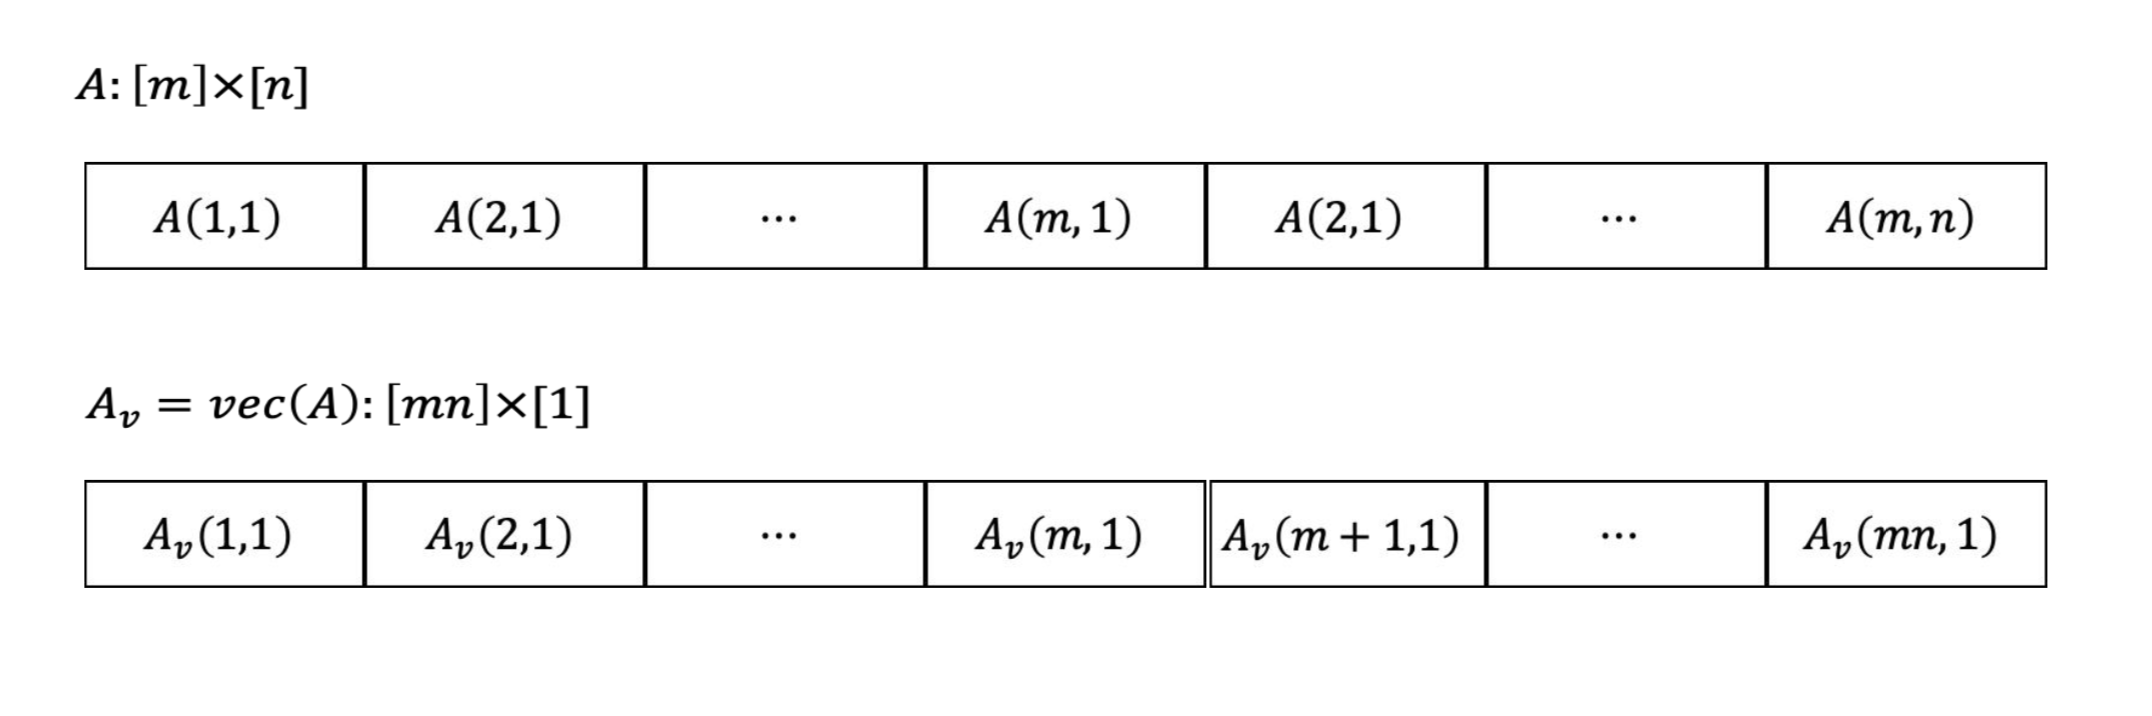
\includegraphics[width=0.7\textwidth]{vec2mat.png}
\caption{$\mathbf{A}$ and vec($\mathbf{A}$) in memory}
\label{Fig:vec2mat}
\end{figure}
\subsubsection{Least Squares Minimization}
As shown in Listing\ref{list:pseudocode}, LSM(Least Squares Minimization) is the main step of the tensor sensing algorithm, which is the most time-consuming part of the entire algorithm. There are many approaches for least squares minimization. QR factorization is one of the most efficient approaches, which is well supported by CUDA.
The least squares problem can be formulated as:
\begin{equation}
\widetilde{\mathbf{x}} = \mathop{\arg \min}_{\mathbf{x}} \| \mathbf{b} - \mathbf{A} \mathbf{x} \|^2_F,
\end{equation}
where $\mathbf{A}$ is a matrix of size $m \times n$, $\mathbf{x}$ is a vector
of size $k \times 1$, and $\mathbf{b}$ is a vector of size $n \times 1$. In the tensor
algorithm, the system we work on is an overdetermined system, where $n >
 k$.
 We perform QR factorization on $\mathbf{A}$ and get $\mathbf{A} = \mathbf{Q}\mathbf{R}$ , where $\mathbf{Q}$ is an
 orthogonal matrix of size $n \times k $ and $\mathbf{R}$ is an upper triangular matrix of size $k \times k$. Taking advantage of the special nature of these matrices we obtain $\mathbf{x}$
as following:
\begin{equation}
\mathbf{x} = \mathbf{R}^{-1}\mathbf{Q}^{T} \ast \mathbf{b}.
\end{equation}

\subsection{Algorithm Optimization on GPU}
\subsubsection{Multiply of Block Diagonal Matrices}
Using the operational properties of the block matrix we get:
\begin{equation}
        [\mathbf{A}_1, \mathbf{A}_2, \cdots, \mathbf{A}_{N_2}]
        \begin{bmatrix}
            \mathbf{U}^c & & & \\
            & \mathbf{U}^c & & \\
            & & \ddots & \\
            & & & \mathbf{U}^c
        \end{bmatrix}
        =
        [\mathbf{A}_1\mathbf{U}^c, \mathbf{A}_2\mathbf{U}^c, \cdots, \mathbf{A}_{N_2}\mathbf{U}^c]
\label{step1}
\end{equation}
It shows that Multiplication of block diagonal matrices can be transformed into a batch of small matrix multiplications. 
As we use column-first format to store $\mathbf{A}$, the batch of $\mathbf{A}_i$ are stored in constant stride. Let $p$ indicate the location of the first element of $\mathbf{A}_0$, then the location of the first element of $\mathbf{A}_i$ is $p+i\times N_1N_3$.  We adopt $cublas<t>gemmStridedBatchd()$ function in cuBlas Library to achieve parallelism of operations.
\begin{figure}[H]
\centering
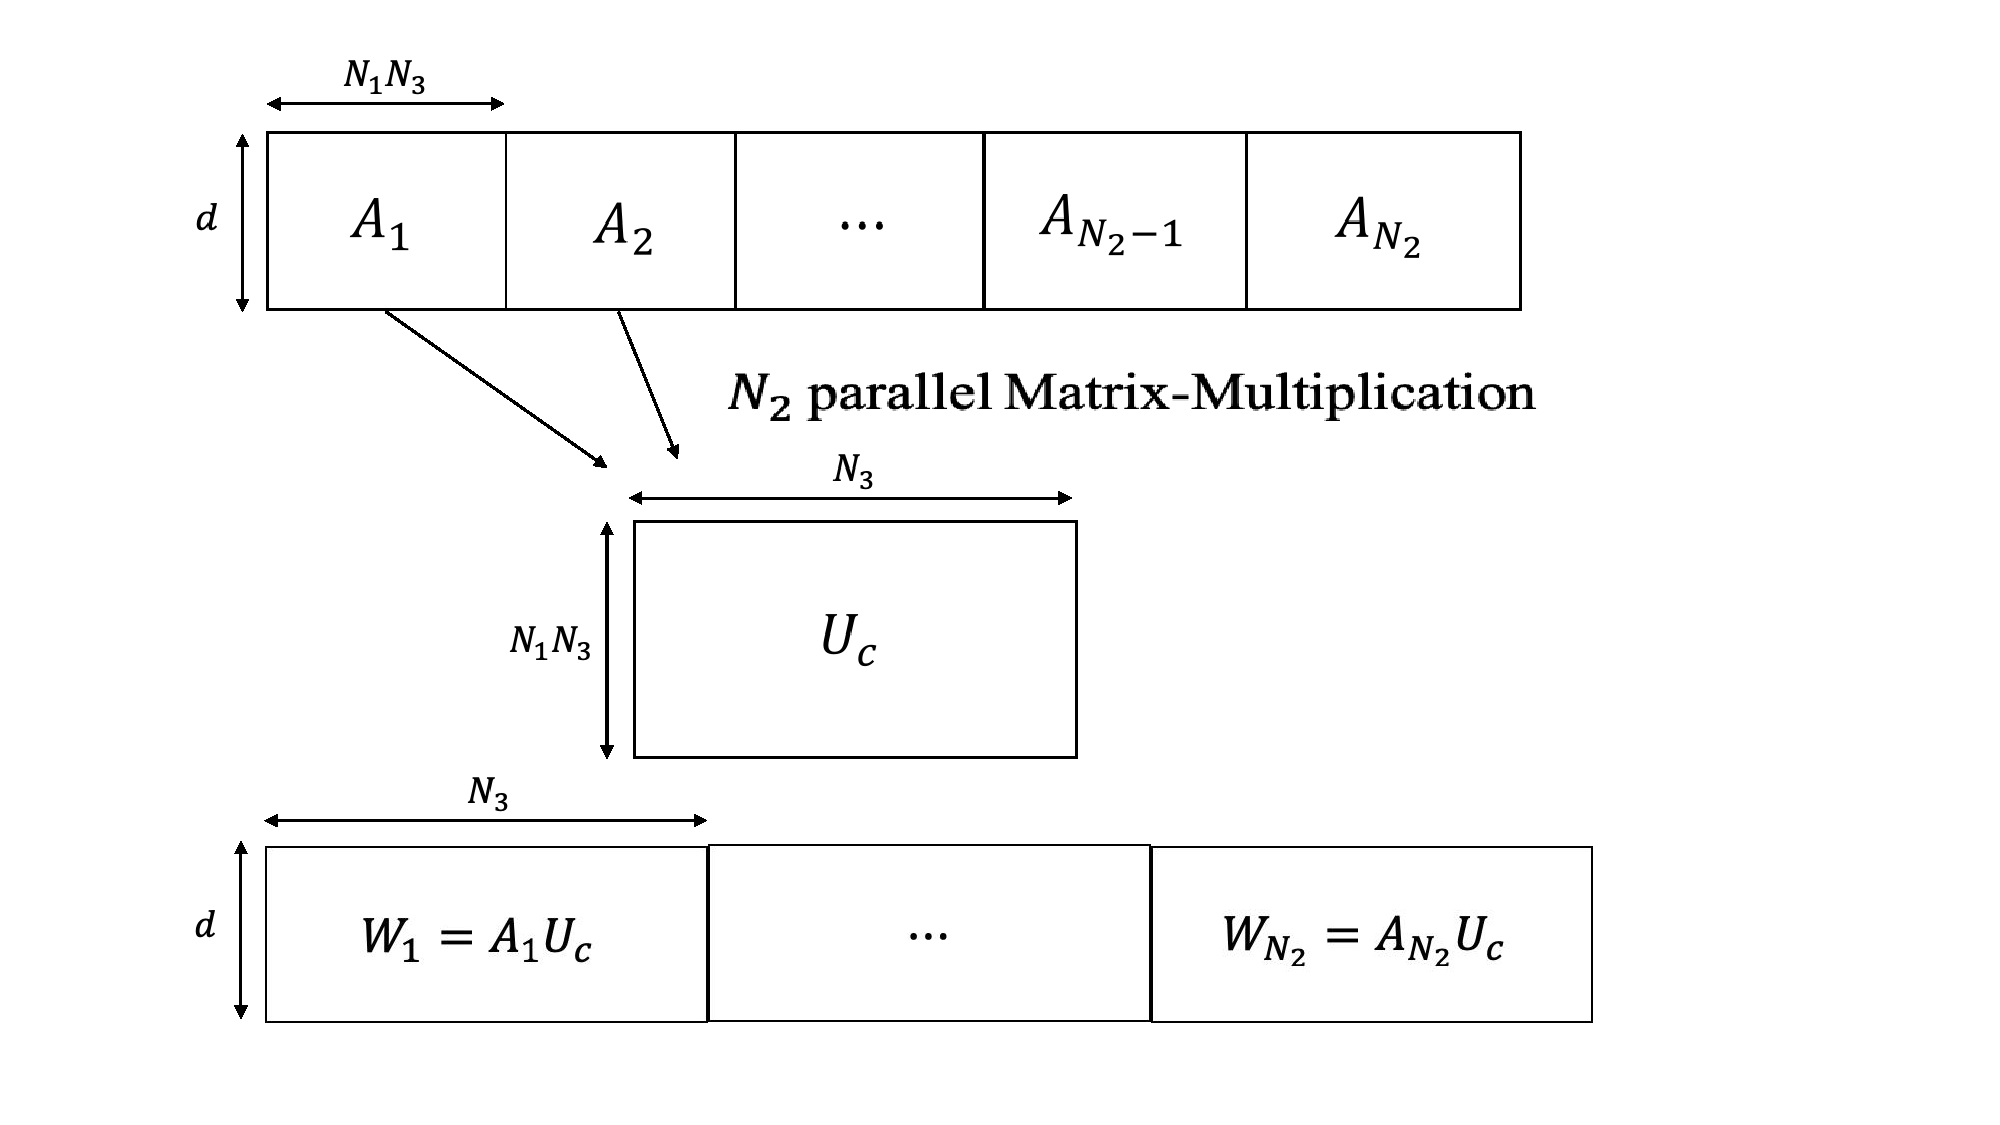
\includegraphics[width=0.7\textwidth]{diagMM.pdf}
\caption{Multiplication of block diagonal matrices on GPU}
\label{Fig:diagMM}
\end{figure}

\begin{table}
\caption{$cublas<t>gemmStridedBatchd$ parameter settings}
\label{tab:gemm}
\begin{tabular}{|l|l|l|}
\hline
Parameters & meaning & value \\
\hline
transA & operation op($\mathbf{A}$) that is non- or transpose & non-transpose \\
\hline
transU & operation op($\mathbf{U}$) that is non- or transpose & transpose \\
\hline
$\mathbf{A}$ & pointer to the $\mathbf{A}$ matrix corresponding to the first instance of the batch & $d_A$ \\
\hline
$\mathbf{U}$ & pointer to the $\mathbf{U}$ matrix & $d_y$ \\
\hline
$\mathbf{W}$ & pointer to the $\mathbf{W}$ matrix & $d_W$ \\
\hline
strideA & the address offset between $\mathbf{A}_i$ and $\mathbf{A}_{i+1}$ & $M\times N_1N_3$ \\
\hline
strideU & the address offset between $\mathbf{U}_i$ and $\mathbf{U}_{i+1}$ & 0 \\
\hline
strideW & the address offset between $\mathbf{W}_i$ and $\mathbf{W}_{i+1}$ & $M\times N_3$ \\
\hline
batchNum & number of $gemm$ to perform in the batch & $N_2$ \\
\hline
\end{tabular}
\end{table}

\subsubsection{Eliminate transpose operations}
We noticed that after each Least Squares method, the transpose of the target matrix is obtained. The transpose operation of the matrix needs to be performed(line 7 and 12), while the transpose operation is quite complicated and will occupy more computing resources.
As the operation after transpose of the matrix is multiplication of diagonal matrices and there is a parameter to control the transpose of the input matrices in the CUDA api $cublas<t>gemmStridedBatchd$, we set the parameter to perform the transpose implicitly.

\subsection{Data reuse and reduce data exchange}
The two main operations in the loop are completed on the device side. Frequent data exchange will seriously affect the efficiency of the program. We use data reuse strategy to reduce data exchange and reduce storage resources occupied on the device side as much as possible.
In the whole loop, we only do two data exchanges. One is that the data is transferred from the CPU to the GPU at the beginning of the loop, and the final result matrix is sent back from the GPU to the CPU.
All intermediate results are covered with new results.One noteworthy thing is that since we use QR decomposition to solve the least squares problem, the input vector $\mathbf{y}$ is covered by the result vector (vec($\mathbf{U}$), vec($\mathbf{V}$)), so we need to reassign the vector $\mathbf{y}$ each time we perform the least squares method. However, it is obviously too time-consuming to read the original data of the vector $\mathbf{y}$ from the CPU every time. In order to solve this problem, we pre-apply a $dyL$ that stores the original data of the vector $\mathbf{y}$. Every time we need to reassign the $dy$, we use the api $cudaMemcpyDeviceToDevice$ . In this way, since the device-to-device assignment is much faster than the data exchange from the CPU to the GPU, at the expense of a small amount of storage space (the space of the vector $\mathbf{y}$ is small compared to the data such as $\mathbf{A}$). ) This is a very good acceleration we have achieved, which will show up in the experimental results in next section.
Alg.\ref{alg:GPU} shows the main CUDA api we adopt and the changes in the memory during the running of the algorithm.

%is that lsm using qr should be mentioned?

\begin{algorithm}
\setstretch{2}
\caption{Tensor Sensing on GPU}
\label{alg:GPU}
\begin{algorithmic}[1]
    \Require data on CPU memory: randomly initialized $\mathbf{U}^0$, measurement vector $\mathbf{y} \in \mathbf{R}^M$, matrix $\mathbf{A} \in \mathbb{R}^{M \times N_1N_2N_3}$ converted from $M$ sensing tensors $\mathcal{A}_m$ and the corresponding transpose matrix $\mathbf{A}_t$
    \Ensure $\mathbf{X}_s \in \mathbb{R}^{N_1N_3 \times N_2}$
    \State apply for memory on GPU device: $dy, dA, dAt , dW, dyL$ ($dA(\mathcal{A})$ means that the content in $dA$ is $\mathcal{A}$, the same below)
    \State data transfer: $\mathcal{A}, \mathcal{A}_t, \mathbf{y}, \mathbf{U}^0 \stackrel{cudaMemcpyHostToDevice}{\longrightarrow} dA(\mathcal{A}), dAt(\mathcal{A}_t), dy(\mathbf{U}^0), dyL(\mathbf{y})$ 
    \For{$i=0 \to IterNum$}
        \State $dW(\text{uninitialized}), dA(\mathcal{A}), dy(\mathbf{U}^i) \stackrel{cublas<t>gemmStridedBatchd}{\longrightarrow} dW(\mathcal{A}\, \text{diag}(\mathbf{U}^i)), dA(\mathcal{A}), dy(\mathbf{U}^i)$
        \State  $dy(\mathbf{U}^i), dyL(\mathbf{y}) \stackrel{cudaMemcpyDeviceToDevice}{\longrightarrow} dy(\mathbf{y}), dyL(\mathbf{y})$
        \State $dW(\mathcal{A}\, \text{diag}(\mathbf{U}^i)), dy(\mathbf{y}) \stackrel{cusolver<t>qr}{\longrightarrow} dy(\mathbf{V}), dW(\text{uninitialized})$
        \State $dW(\text{uninitialized}, dAt(\mathcal{A}_t), dy(\mathbf{V}^i)) \stackrel{cublas<t>gemmStridedBatchd}{\longrightarrow} dW(\mathcal{A}_t\, \text{diag}(\mathbf{V}^i)), dAt(\mathcal{A}_t), dy(\mathbf{V}^i)$
        \State  $dy(\mathbf{V}^i), dyL(\mathbf{y}) \stackrel{cudaMemcpyDeviceToDevice}{\longrightarrow} dy(\mathbf{y}), dyL(\mathbf{y})$
        \State $dW(\mathcal{A}_t\, \text{diag}(\mathbf{V}^i)), dy(\mathbf{y}) \stackrel{cusolver<t>qr}{\longrightarrow} dy(\mathbf{U}^i), dW(\text{uninitialized})$
    \EndFor
    \State \Return $\mathbf{X}^s = \mathbf{U}\mathbf{V}$
\end{algorithmic}
\end{algorithm}

\section{Experiment Methodology}
In this section, we describe the experiment methodology including the hardware and software platform, testing data, testing process, and the comparison metrics.

\subsection{Hardware and Software Platform}
We use an NVIDIA Tesla V100 GPU card to evaluate performance of the method we propose. Tesla V100 is powered by NVIDIA Volta architecvture, comes in 32GB configuration. It is intalled on a server with 128 GB memory and an Intel i7-7820x CPU clocked at 3.6 GHz containing, which contains eight cores and supports 16 hardware threads with hyperthreading. The server is running Ubuntu 18.04.1 LTS with the kernel version 4.15.0. There is a Matlab R2017b installed that executes the CPU implementation in previous work as the baseline for comparison with our method. NVIDIA CUDA 10.0 is used in all experiments of our method execution.
\subsection{Testing Data}
In the experiment, we use both synthetic and real datasets to test our method. The synthetic data is generated according to the compressed sensing\cite{matsuda2017multi}. For real dataset, we use a IKEA 3D dataset that generate a ground truth tensor of size $40 \times 40 \times 6$ with $\mathcal{L}$-rank 1.

\subsection{Testing Process}
The synthetic and real datasets are processed by the Matlab code on CPUs and our method on GPUs, respectively. We repeat each experiment five times and report the average results.

\subsection{Comparison Metrics}
We compare the CPU algorithm with the GPU algorithm in two metrics: running time, relative error rate.
\begin{itemize}
    \item \textit{running time:} varying the tensor size and fixing other parameter, we measure the execution time of original CPU method, GPU implementation without optimization and our final accelerated method. Finally we calculate speedups as the CPU time divided by our method on GPU time.
    \item \textit{error rate:} we adopt the metric relative square error, defined as $ RSE = \| \widehat{\mathcal{X}} - \mathcal{X} \|_F / \|\mathcal{X} \|_F $.
\end{itemize}

\section{Results and Analysis}
\subsection{Running time of Synthetic Data}
\begin{figure}[t]
    \centering
    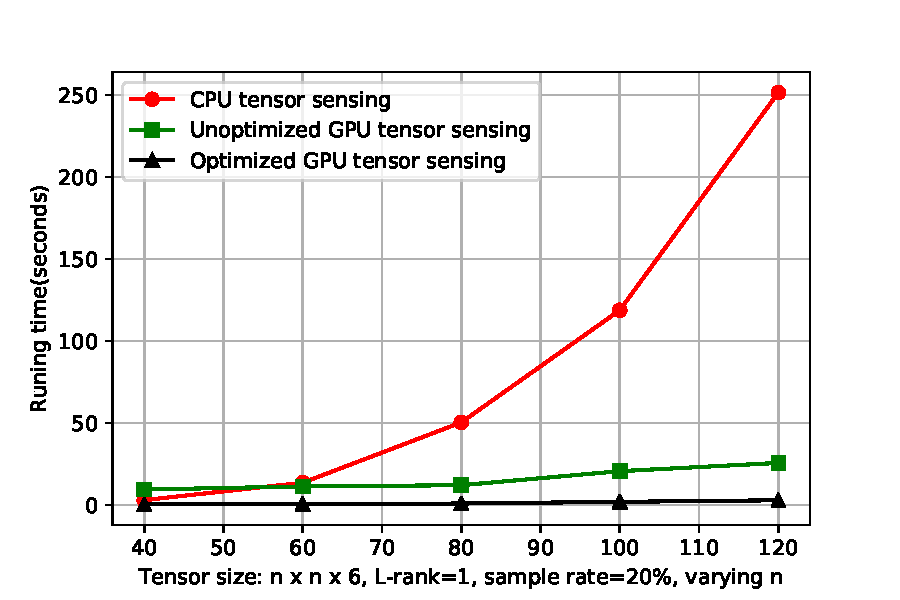
\includegraphics[width=3.5in]{runtime.pdf}
    \caption{Running time of CPU algorithm and GPU algorithm}
    \label{pic:runtime}
\end{figure}

\begin{table}[t]
  \renewcommand{\arraystretch}{1.3}
  \centering
  \scriptsize
  \caption{Running time under different tensor size ($n \times n \times 6$).}
  \begin{tabular}{|l|l|l|l|l|l|}
    \hline
    \textbf{\textbf{n}} & \textbf{40}& \textbf{60}& \textbf{80} & \textbf{100} & \textbf{120}\\
    \hline
    CPU time(S) & 3.07 & 13.65 & 50.43 & 118.84 & 251.54\\
    \hline
    GPU without optimization time(S) & 9.50 & 11.40 & 12.15 & 20.70 & 25.74\\
    \hline
    GPU with optimization time(S) & 0.44 & 0.63 & 0.98 & 2.01 & 2.97\\
    \hline
    Speedups & 6.98 & 21.67 & 51.46 & 59.12 & 84.70\\
    \hline
  \end{tabular}
  \label{tbl_runtime}
\end{table}

Fig.\ref{pic:runtime} shows that the running time of the two GPU implementations and the CPU implementation for $\mathcal{X}$ of size $n\times n \times 6$ of $\mathcal{L}$-rank 1, where $n$ varies from 40 to 120 at a step of 20. The sampling rate is set to 20\%, and both CPU and GPU algorithms iterate 5 itrations for completion. The detailed time value is listed in \ref{tbl_runtime}. 
While $M = N_1 \times N_2 \times N_3 \times \text{sampling rate}$ and $\mathcal{A} \in \mathbb{R}^{M \times N_1N_2N_3}$, the scale of the main operation matrix $\mathcal{A}$ increases at a rate four times the rate of increase of $n$. 
It can be seen that the run time of the CPU method without any parallel strategy is polynomial with the increase of n, and both GPU implementations are linearly changed. As for GPU implementation without data reuse, when the matrix size is small, the data exchange takes up most of the running time and the running time is even longer than the CPU implementation. 
As for our final method, which is with data reuse and other parallel acceleration strategy, it achieves a good speedup at all scales and allows for greater speedups in larger data sizes where GPU memory is allowed.
\begin{figure}[t]
    \centering
    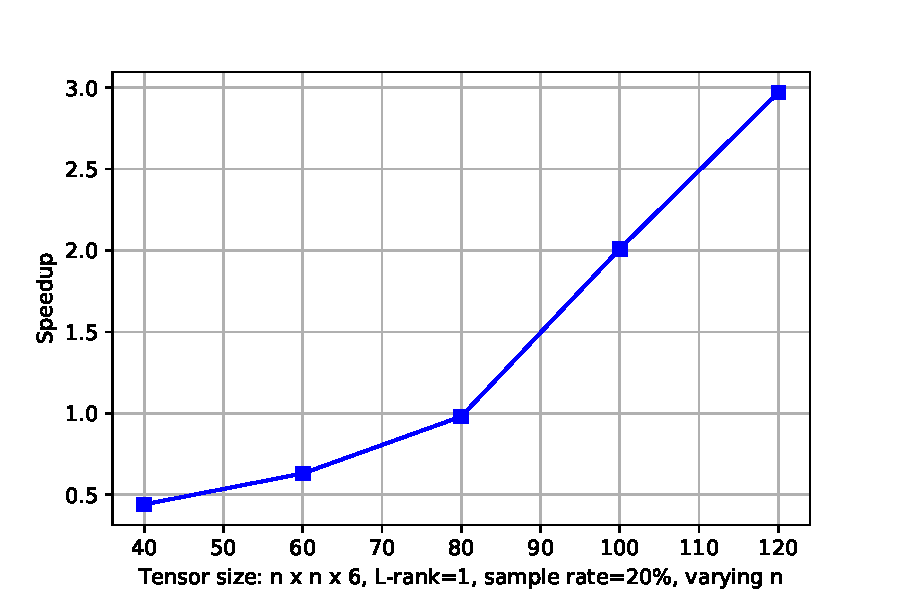
\includegraphics[width=3.5in]{speedup.pdf}
    \caption{Speedups of CPU implementation and GPU implementation}
    \label{pic:runtime}
\end{figure}

\subsection{Error Rate and Running Time of Real Data}
\begin{figure}[t]
    \centering
    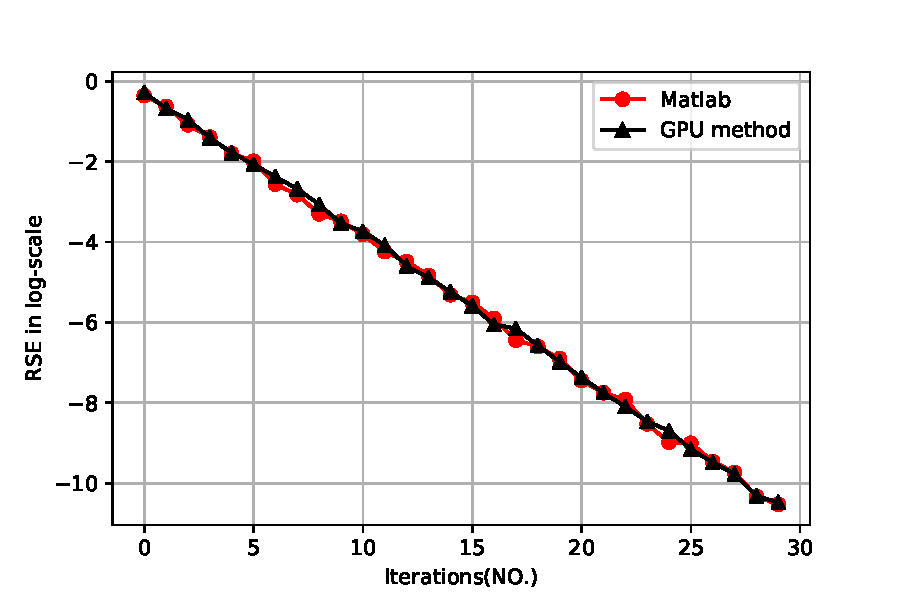
\includegraphics[width=3.5in]{rse.pdf}
    \caption{RSE of CPU implementation and GPU implementation}
    \label{pic:rse}
\end{figure}

This experiment compares the error rate if the CPU and GPU implementation under different iterations for $\mathcal{X}$ of size $40 \times 40 \times 6$ with $\mathcal{L}$-rank 1. The sampling rate is set to 50\%. The running time of the CPU algorithm is about 15 seconds, while the running time of the GPU algorithm is about 1 second. As shown in Fig. \ref{pic:rse}, when iteration varies from 1 to 30, the RSEs drop significantly. More importantly, the origin CPU implementation and the GPU implementation achieve almost the same RSEs at all iterations (the two curves in Fig. \ref{pic:rse} overlap), which means that the two implementations have similar error rate performance in tensor sensing.

\section{Conclusions}

This section is not mandatory, but can be added to the manuscript if the discussion is unusually long or complex.

%%%%%%%%%%%%%%%%%%%%%%%%%%%%%%%%%%%%%%%%%%
\section{Patents}
This section is not mandatory, but may be added if there are patents resulting from the work reported in this manuscript.

%%%%%%%%%%%%%%%%%%%%%%%%%%%%%%%%%%%%%%%%%%
\vspace{6pt} 

%%%%%%%%%%%%%%%%%%%%%%%%%%%%%%%%%%%%%%%%%%
%% optional
%\supplementary{The following are available online at \linksupplementary{s1}, Figure S1: title, Table S1: title, Video S1: title.}

% Only for the journal Methods and Protocols:
% If you wish to submit a video article, please do so with any other supplementary material.
% \supplementary{The following are available at \linksupplementary{s1}, Figure S1: title, Table S1: title, Video S1: title. A supporting video article is available at doi: link.}

%%%%%%%%%%%%%%%%%%%%%%%%%%%%%%%%%%%%%%%%%%
\authorcontributions{For research articles with several authors, a short paragraph specifying their individual contributions must be provided. The following statements should be used “conceptualization, X.X. and Y.Y.; methodology, X.X.; software, X.X.; validation, X.X., Y.Y. and Z.Z.; formal analysis, X.X.; investigation, X.X.; resources, X.X.; data curation, X.X.; writing—original draft preparation, X.X.; writing—review and editing, X.X.; visualization, X.X.; supervision, X.X.; project administration, X.X.; funding acquisition, Y.Y.”, please turn to the  \href{http://img.mdpi.org/data/contributor-role-instruction.pdf}{CRediT taxonomy} for the term explanation. Authorship must be limited to those who have contributed substantially to the work reported.}

%%%%%%%%%%%%%%%%%%%%%%%%%%%%%%%%%%%%%%%%%%
\funding{Please add: ``This research received no external funding'' or ``This research was funded by NAME OF FUNDER grant number XXX.'' and  and ``The APC was funded by XXX''. Check carefully that the details given are accurate and use the standard spelling of funding agency names at \url{https://search.crossref.org/funding}, any errors may affect your future funding.}

%%%%%%%%%%%%%%%%%%%%%%%%%%%%%%%%%%%%%%%%%%
\acknowledgments{In this section you can acknowledge any support given which is not covered by the author contribution or funding sections. This may include administrative and technical support, or donations in kind (e.g., materials used for experiments).}

%%%%%%%%%%%%%%%%%%%%%%%%%%%%%%%%%%%%%%%%%%
\conflictsofinterest{Declare conflicts of interest or state ``The authors declare no conflict of interest.'' Authors must identify and declare any personal circumstances or interest that may be perceived as inappropriately influencing the representation or interpretation of reported research results. Any role of the funders in the design of the study; in the collection, analyses or interpretation of data; in the writing of the manuscript, or in the decision to publish the results must be declared in this section. If there is no role, please state ``The funders had no role in the design of the study; in the collection, analyses, or interpretation of data; in the writing of the manuscript, or in the decision to publish the results''.} 

%%%%%%%%%%%%%%%%%%%%%%%%%%%%%%%%%%%%%%%%%%
%% optional
\abbreviations{The following abbreviations are used in this manuscript:\\

\noindent 
\begin{tabular}{@{}ll}
MDPI & Multidisciplinary Digital Publishing Institute\\
DOAJ & Directory of open access journals\\
TLA & Three letter acronym\\
LD & linear dichroism
\end{tabular}}

%%%%%%%%%%%%%%%%%%%%%%%%%%%%%%%%%%%%%%%%%%
%% optional
\appendixtitles{no} %Leave argument "no" if all appendix headings stay EMPTY (then no dot is printed after "Appendix A"). If the appendix sections contain a heading then change the argument to "yes".
\appendixsections{multiple} %Leave argument "multiple" if there are multiple sections. Then a counter is printed ("Appendix A"). If there is only one appendix section then change the argument to "one" and no counter is printed ("Appendix").
\appendix
\section{}
\unskip
\subsection{}
The appendix is an optional section that can contain details and data supplemental to the main text. For example, explanations of experimental details that would disrupt the flow of the main text, but nonetheless remain crucial to understanding and reproducing the research shown; figures of replicates for experiments of which representative data is shown in the main text can be added here if brief, or as Supplementary data. Mathematical proofs of results not central to the paper can be added as an appendix.

\section{}
All appendix sections must be cited in the main text. In the appendixes, Figures, Tables, etc. should be labeled starting with `A', e.g., Figure A1, Figure A2, etc. 

%%%%%%%%%%%%%%%%%%%%%%%%%%%%%%%%%%%%%%%%%%
% Citations and References in Supplementary files are permitted provided that they also appear in the reference list here. 

%=====================================
% References, variant A: internal bibliography
%=====================================
\reftitle{References}
%\begin{thebibliography}{999}
% Reference 1
%\bibitem[Author1(year)]{ref-journal}
%Author1, T. The title of the cited article. {\em Journal Abbreviation} {\bf 2008}, {\em 10}, 142-149, doi:xxxxx.
% Reference 2
%\bibitem[Author2(year)]{ref-book}
%Author2, L. The title of the cited contribution. In {\em The Book Title}; Editor1, F., Editor2, A., Eds.; Publishing House: City, Country, 2007; pp. 32-58, ISBN.
%\end{thebibliography}

% The following MDPI journals use author-date citation: Arts, Econometrics, Economies, Genealogy, Humanities, IJFS, JRFM, Laws, Religions, Risks, Social Sciences. For those journals, please follow the formatting guidelines on http://www.mdpi.com/authors/references
% To cite two works by the same author: \citeauthor{ref-journal-1a} (\citeyear{ref-journal-1a}, \citeyear{ref-journal-1b}). This produces: Whittaker (1967, 1975)
% To cite two works by the same author with specific pages: \citeauthor{ref-journal-3a} (\citeyear{ref-journal-3a}, p. 328; \citeyear{ref-journal-3b}, p.475). This produces: Wong (1999, p. 328; 2000, p. 475)

%=====================================
% References, variant B: external bibliography
%=====================================
\externalbibliography{yes}
\bibliography{mybibfile}

%%%%%%%%%%%%%%%%%%%%%%%%%%%%%%%%%%%%%%%%%%
%% optional

%% for journal Sci
%\reviewreports{\\
%Reviewer 1 comments and authors’ response\\
%Reviewer 2 comments and authors’ response\\
%Reviewer 3 comments and authors’ response
%}

%%%%%%%%%%%%%%%%%%%%%%%%%%%%%%%%%%%%%%%%%%
\end{document}
